% ============================================================
% 初升高衔接讲义四：平面几何证明综合
% 编译命令：xelatex -interaction=nonstopmode 衔接4_平面几何证明综合.tex
% ============================================================
\documentclass[12pt, a4paper]{ctexart}
\usepackage[margin=2.2cm]{geometry}
\usepackage{amsmath, amssymb}
\usepackage{enumitem}
\usepackage{tcolorbox}
\usepackage{booktabs}
\usepackage{array}
\usepackage{fancyhdr}
\usepackage{xcolor}
\usepackage{tikz}
\usepackage{hyperref}
\usepackage{graphicx}
\usepackage{multirow}
\usepackage{pgfplots}
\usepackage{amsthm}
\pgfplotsset{compat=1.18}
\usetikzlibrary{angles, quotes, patterns, decorations.markings, calc, intersections, arrows.meta}

% 颜色定义
\definecolor{mainblue}{RGB}{41, 98, 168}
\definecolor{lightblue}{RGB}{230, 240, 255}
\definecolor{tipgreen}{RGB}{34, 139, 87}
\definecolor{lightgreen}{RGB}{235, 250, 240}
\definecolor{warnred}{RGB}{200, 50, 50}
\definecolor{lightred}{RGB}{255, 240, 240}
\definecolor{examorange}{RGB}{210, 120, 20}
\definecolor{lightorange}{RGB}{255, 248, 235}
\definecolor{apppurple}{RGB}{120, 60, 170}
\definecolor{lightpurple}{RGB}{245, 238, 255}
\definecolor{dashgray}{RGB}{120, 120, 120}

% 页眉页脚
\pagestyle{fancy}
\fancyhf{}
\fancyhead[L]{\small\textcolor{mainblue}{\textbf{初升高衔接 · 平面几何证明}}}
\fancyhead[R]{\small\textcolor{mainblue}{衔接讲义四}}
\fancyfoot[C]{\small —\ \thepage\ —}
\renewcommand{\headrulewidth}{0.6pt}
\renewcommand{\headrule}{\hbox to\headwidth{\color{mainblue}\leaders\hrule height \headrulewidth\hfill}}
\renewcommand{\footrulewidth}{0pt}

% tcolorbox 样式
\newtcolorbox{knowledgebox}[1][]{%
  colback=lightblue, colframe=mainblue,
  fonttitle=\bfseries\large, title=#1,
  arc=3mm, boxrule=0.8pt,
  left=8pt, right=8pt, top=6pt, bottom=6pt
}

\newtcolorbox{tipbox}[1][]{%
  colback=lightgreen, colframe=tipgreen,
  fonttitle=\bfseries, title=#1,
  arc=2mm, boxrule=0.6pt,
  left=6pt, right=6pt, top=4pt, bottom=4pt
}

\newtcolorbox{warnbox}[1][]{%
  colback=lightred, colframe=warnred,
  fonttitle=\bfseries, title=#1,
  arc=2mm, boxrule=0.6pt,
  left=6pt, right=6pt, top=4pt, bottom=4pt
}

\newtcolorbox{examplebox}[1][]{%
  colback=lightorange, colframe=examorange,
  fonttitle=\bfseries, title=#1,
  arc=3mm, boxrule=0.8pt,
  left=8pt, right=8pt, top=6pt, bottom=6pt
}

\newtcolorbox{appbox}[1][]{%
  colback=lightpurple, colframe=apppurple,
  fonttitle=\bfseries, title=#1,
  arc=3mm, boxrule=0.8pt,
  left=8pt, right=8pt, top=6pt, bottom=6pt
}

\setCJKmainfont{Hiragino Sans GB}
\setCJKsansfont{Heiti SC}

% 标记命令
\newcommand{\markangle}[3]{\widehat{#1#2#3}}

\begin{document}

% ============ 标题页 ============
\begin{center}
{\Huge\bfseries\textcolor{mainblue}{平面几何证明综合}}\\[12pt]
{\Large\textcolor{gray}{初升高衔接讲义}}\\[8pt]
\rule{0.6\textwidth}{1pt}\\[8pt]
{\normalsize 适用：初升高衔接\quad |\quad 课时：4--5课时}
\end{center}
\vspace{6pt}

\begin{knowledgebox}[写在前面]
平面几何证明是高中数学（尤其是立体几何）的重要基础。高中立体几何中的许多证明题，都需要在平面内先完成全等或相似的推理。本讲义系统回顾初中阶段最核心的平面几何证明方法，帮助同学们在进入高中前夯实基础。

\medskip
\noindent\textbf{学习建议：}
\begin{enumerate}[leftmargin=2em]
  \item 先回顾知识点，确保每条判定定理都能\textbf{脱口而出}；
  \item 例题要自己先想一想，再看解答，重点体会\textbf{思路}而非背步骤；
  \item 课堂练习独立完成，写好\textbf{完整的证明过程}；
  \item 高中立体几何的"线面平行""线面垂直"证明，本质上都归结为\textbf{平面几何证明}。
\end{enumerate}
\end{knowledgebox}

\vspace{4pt}

% ============================================================
%  第一部分：知识点讲解
% ============================================================
\section*{\textcolor{mainblue}{一、知识点讲解}}

% ---- 1.1 全等三角形 ----
\subsection*{1.1\quad 全等三角形判定与性质回顾}

\begin{knowledgebox}[全等三角形的性质]
若 $\triangle ABC \cong \triangle DEF$，则：
\begin{enumerate}[nosep]
  \item \textbf{对应边相等：}$AB=DE$，$BC=EF$，$AC=DF$；
  \item \textbf{对应角相等：}$\angle A=\angle D$，$\angle B=\angle E$，$\angle C=\angle F$。
\end{enumerate}

\begin{center}
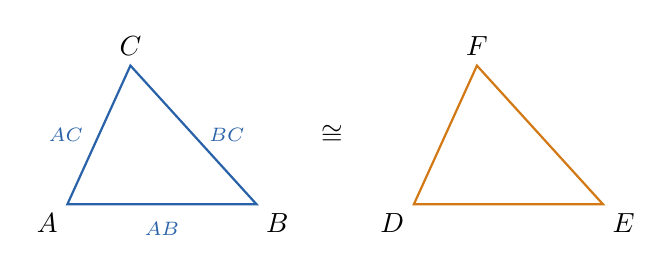
\begin{tikzpicture}[scale=0.8]
  \coordinate (A) at (0,0);
  \coordinate (B) at (3,0);
  \coordinate (C) at (1,2.2);
  \draw[thick, mainblue] (A)--(B)--(C)--cycle;
  \node[below left] at (A) {$A$};
  \node[below right] at (B) {$B$};
  \node[above] at (C) {$C$};
  \node[mainblue] at (1.5,-0.4) {$\scriptstyle AB$};
  \node[mainblue, right] at (2.1,1.1) {$\scriptstyle BC$};
  \node[mainblue, left] at (0.4,1.1) {$\scriptstyle AC$};

  \node at (4.2,1.1) {$\cong$};

  \coordinate (D) at (5.5,0);
  \coordinate (E) at (8.5,0);
  \coordinate (F) at (6.5,2.2);
  \draw[thick, examorange] (D)--(E)--(F)--cycle;
  \node[below left] at (D) {$D$};
  \node[below right] at (E) {$E$};
  \node[above] at (F) {$F$};
\end{tikzpicture}
\end{center}
\end{knowledgebox}

\begin{knowledgebox}[全等三角形的五种判定方法]
\begin{center}
\renewcommand{\arraystretch}{1.5}
\begin{tabular}{|c|c|c|}
\hline
\textbf{判定} & \textbf{条件} & \textbf{说明} \\
\hline
SSS & 三边对应相等 & 最"朴素"的判定 \\
\hline
SAS & 两边及\textbf{夹角}对应相等 & \textcolor{warnred}{角必须是夹角！} \\
\hline
ASA & 两角及\textbf{夹边}对应相等 & 边必须是夹边 \\
\hline
AAS & 两角及\textbf{一角的对边}对应相等 & 由 ASA + 三角形内角和推出 \\
\hline
HL & 斜边和一条直角边对应相等 & \textcolor{warnred}{仅限直角三角形} \\
\hline
\end{tabular}
\end{center}

\begin{warnbox}[易错提醒]
\begin{itemize}[nosep]
  \item \textbf{SSA 不能判定全等！}两边和其中一边的对角相等，不能保证两个三角形全等。
  \item \textbf{AAA 不能判定全等！}三个角对应相等只能说明两个三角形\textbf{相似}，不能说明全等。
  \item 写证明时，对应顶点必须写在对应位置，如 $\triangle ABC \cong \triangle DEF$ 表示 $A\leftrightarrow D$，$B\leftrightarrow E$，$C\leftrightarrow F$。
\end{itemize}
\end{warnbox}
\end{knowledgebox}

% ---- 1.2 相似三角形 ----
\subsection*{1.2\quad 相似三角形判定与性质回顾}

\begin{knowledgebox}[相似三角形的性质]
若 $\triangle ABC \sim \triangle DEF$，相似比为 $k$（即 $\dfrac{AB}{DE}=\dfrac{BC}{EF}=\dfrac{AC}{DF}=k$），则：
\begin{enumerate}[nosep]
  \item \textbf{对应角相等：}$\angle A=\angle D$，$\angle B=\angle E$，$\angle C=\angle F$；
  \item \textbf{对应边成比例：}$\dfrac{AB}{DE}=\dfrac{BC}{EF}=\dfrac{AC}{DF}$。
\end{enumerate}
\end{knowledgebox}

\begin{knowledgebox}[相似三角形的三种判定方法]
\begin{center}
\renewcommand{\arraystretch}{1.5}
\begin{tabular}{|c|c|c|}
\hline
\textbf{判定} & \textbf{条件} & \textbf{说明} \\
\hline
AA & 两角对应相等 & 最常用，只需找两对角 \\
\hline
SAS（相似） & 两边对应成比例且\textbf{夹角}相等 & 注意与全等 SAS 的类比 \\
\hline
SSS（相似） & 三边对应成比例 & 注意与全等 SSS 的类比 \\
\hline
\end{tabular}
\end{center}

\begin{tipbox}[规律总结]
在实际题目中，\textbf{AA 判定}使用频率最高。常见策略：
\begin{itemize}[nosep]
  \item 找\textbf{公共角}（两三角形共用一个角）；
  \item 找\textbf{对顶角}；
  \item 找\textbf{平行线}产生的同位角或内错角。
\end{itemize}
只要再找到一对角相等，就能用 AA 证相似。
\end{tipbox}
\end{knowledgebox}

% ---- 1.3 相似比与面积比 ----
\subsection*{1.3\quad 相似比与面积比的关系}

\begin{knowledgebox}[相似比、周长比与面积比]
若 $\triangle ABC \sim \triangle DEF$，相似比为 $k$，则：
\begin{enumerate}[nosep]
  \item \textbf{周长比} $=$ 相似比 $= k$；
  \item \textbf{面积比} $=$ 相似比的平方 $= k^2$。
\end{enumerate}

\medskip
\textbf{推广：}对于相似多边形，上述关系同样成立。

\begin{center}
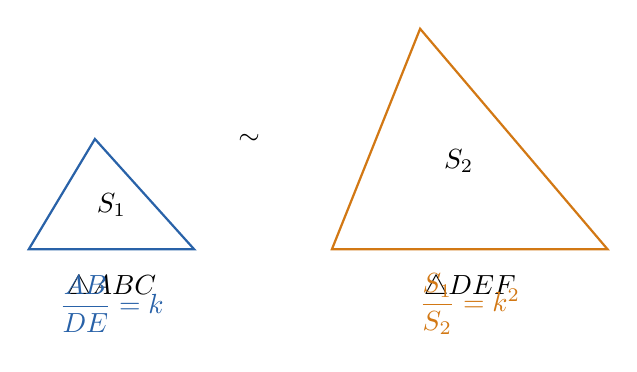
\begin{tikzpicture}[scale=0.7]
  % 小三角形
  \coordinate (A) at (0,0);
  \coordinate (B) at (3,0);
  \coordinate (C) at (1.2,2);
  \draw[thick, mainblue] (A)--(B)--(C)--cycle;
  \node[below] at (1.5,-0.3) {$\triangle ABC$};
  \node at (1.5,0.8) {$S_1$};
  % 大三角形
  \coordinate (D) at (5.5,0);
  \coordinate (E) at (10.5,0);
  \coordinate (F) at (7.1,4);
  \draw[thick, examorange] (D)--(E)--(F)--cycle;
  \node[below] at (8,-0.3) {$\triangle DEF$};
  \node at (7.8,1.6) {$S_2$};
  % 标注
  \node at (4,2) {$\sim$};
  \node[mainblue] at (1.5,-1) {$\dfrac{AB}{DE}=k$};
  \node[examorange] at (8,-1) {$\dfrac{S_1}{S_2}=k^2$};
\end{tikzpicture}
\end{center}

\begin{warnbox}[易错提醒]
面积比是相似比的\textbf{平方}，不是相似比本身！若相似比为 $2:3$，则面积比为 $4:9$，而非 $2:3$。
\end{warnbox}
\end{knowledgebox}

% ---- 1.4 四边形 ----
\subsection*{1.4\quad 平行四边形 / 矩形 / 菱形 / 正方形}

\begin{knowledgebox}[特殊四边形的性质与判定]

\textbf{一、平行四边形}

\begin{minipage}{0.48\textwidth}
\textbf{性质：}
\begin{itemize}[nosep]
  \item 对边平行且相等
  \item 对角相等
  \item 邻角互补
  \item 对角线互相平分
\end{itemize}
\end{minipage}
\hfill
\begin{minipage}{0.48\textwidth}
\textbf{判定（5种）：}
\begin{itemize}[nosep]
  \item 两组对边分别平行
  \item 两组对边分别相等
  \item 一组对边平行且相等
  \item 两条对角线互相平分
  \item 两组对角分别相等
\end{itemize}
\end{minipage}

\begin{center}
\begin{tikzpicture}[scale=0.7]
  \coordinate (A) at (0,2);
  \coordinate (B) at (4,2);
  \coordinate (C) at (5,0);
  \coordinate (D) at (1,0);
  \draw[thick, mainblue] (A)--(B)--(C)--D--cycle;
  \draw[thick, dashed, dashgray] (A)--(C);
  \draw[thick, dashed, dashgray] (B)--(D);
  \coordinate (O) at (intersection of A--C and B--D);
  \fill (O) circle (1.5pt);
  \node[above left] at (A) {$A$};
  \node[above right] at (B) {$B$};
  \node[below right] at (C) {$C$};
  \node[below left] at (D) {$D$};
  \node[below right] at (O) {$O$};
\end{tikzpicture}
\end{center}

\textbf{二、矩形（有一个角是直角的平行四边形）}

\begin{itemize}[nosep]
  \item 具有平行四边形的\textbf{所有性质}；
  \item 四个角都是直角；
  \item 对角线\textbf{相等}且互相平分。
\end{itemize}

\textbf{三、菱形（有一组邻边相等的平行四边形）}

\begin{itemize}[nosep]
  \item 具有平行四边形的\textbf{所有性质}；
  \item 四条边都相等；
  \item 对角线互相\textbf{垂直}平分，且每条对角线平分一组对角。
\end{itemize}

\textbf{四、正方形（既是矩形又是菱形）}

\begin{itemize}[nosep]
  \item 具有矩形和菱形的\textbf{所有性质}；
  \item 四条边相等，四个角都是直角；
  \item 对角线相等、互相垂直平分。
\end{itemize}

\begin{center}
\begin{tikzpicture}[scale=0.8]
  % 矩形
  \draw[thick, mainblue] (0,0) rectangle (2.5,1.5);
  \node at (1.25,-0.3) {矩形};
  \draw[thick, dashed, dashgray] (0,0)--(2.5,1.5);
  \draw[thick, dashed, dashgray] (2.5,0)--(0,1.5);
  % 菱形
  \draw[thick, tipgreen] (4.5,0.75)--(5.75,1.5)--(7,0.75)--(5.75,0)--cycle;
  \node at (5.75,-0.3) {菱形};
  \draw[thick, dashed, dashgray] (4.5,0.75)--(7,0.75);
  \draw[thick, dashed, dashgray] (5.75,1.5)--(5.75,0);
  % 正方形
  \draw[thick, examorange] (9,0) rectangle (11,2);
  \node at (10,-0.3) {正方形};
  \draw[thick, dashed, dashgray] (9,0)--(11,2);
  \draw[thick, dashed, dashgray] (11,0)--(9,2);
\end{tikzpicture}
\end{center}
\end{knowledgebox}

% ---- 1.5 辅助线技巧 ----
\subsection*{1.5\quad 常用辅助线技巧回顾}

\begin{knowledgebox}[三种常用辅助线]

\textbf{一、倍长中线法}

当题目出现\textbf{中线}（或中点）时，将中线延长一倍，构造全等三角形。

\begin{center}
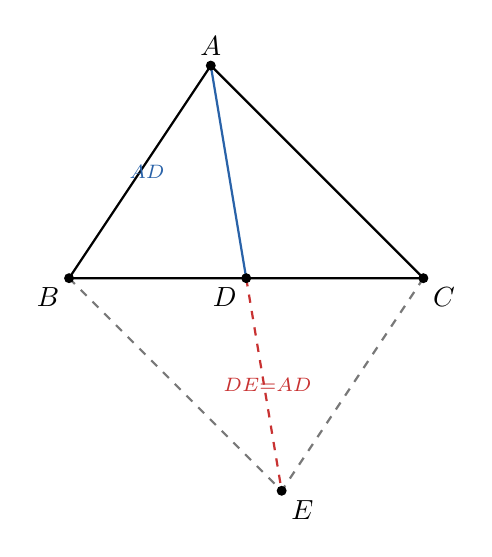
\begin{tikzpicture}[scale=0.9]
  \coordinate (A) at (2,3);
  \coordinate (B) at (0,0);
  \coordinate (C) at (5,0);
  \coordinate (D) at (2.5,0);
  \coordinate (E) at (3,-3);
  \draw[thick] (A)--(B)--(C)--cycle;
  \draw[thick, mainblue] (A)--(D);
  \draw[thick, dashed, warnred] (D)--(E);
  \draw[thick, dashed, dashgray] (B)--(E);
  \draw[thick, dashed, dashgray] (C)--(E);
  \fill (A) circle (2pt) node[above] {$A$};
  \fill (B) circle (2pt) node[below left] {$B$};
  \fill (C) circle (2pt) node[below right] {$C$};
  \fill (D) circle (2pt) node[below left] {$D$};
  \fill (E) circle (2pt) node[below right] {$E$};
  \node[mainblue] at (1.1,1.5) {$\scriptstyle AD$};
  \node[warnred] at (2.8,-1.5) {$\scriptstyle DE=AD$};
\end{tikzpicture}
\end{center}

$\triangle ADB \cong \triangle EDC$（SAS），从而 $AB=EC$，实现线段转移。

\medskip
\textbf{二、截长补短法}

证明线段\textbf{和差关系}（如 $a=b+c$）时使用。

\begin{itemize}[nosep]
  \item \textbf{截长：}在长线段上截取一段等于短线段，证剩余部分等于另一短线段。
  \item \textbf{补短：}将短线段延长，使总长等于长线段，证延长部分等于另一短线段。
\end{itemize}

\medskip
\textbf{三、作平行线法}

当需要构造\textbf{相似三角形}或利用\textbf{平行线分线段成比例}时，过某点作已知直线的平行线。

\begin{center}
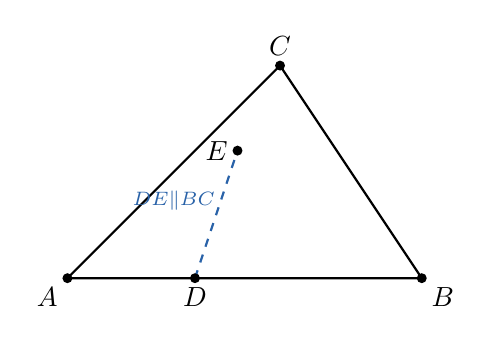
\begin{tikzpicture}[scale=0.9]
  \coordinate (A) at (0,0);
  \coordinate (B) at (5,0);
  \coordinate (C) at (3,3);
  \coordinate (D) at (1.8,0);
  \coordinate (E) at (2.4,1.8);
  \draw[thick] (A)--(B)--(C)--cycle;
  \draw[thick, mainblue, dashed] (D)--(E);
  \fill (A) circle (2pt) node[below left] {$A$};
  \fill (B) circle (2pt) node[below right] {$B$};
  \fill (C) circle (2pt) node[above] {$C$};
  \fill (D) circle (2pt) node[below] {$D$};
  \fill (E) circle (2pt) node[left] {$E$};
  \node[mainblue] at (1.5,1.1) {$\scriptstyle DE\parallel BC$};
\end{tikzpicture}
\end{center}

$DE \parallel BC \Rightarrow \triangle ADE \sim \triangle ABC$，得到比例关系。

\end{knowledgebox}

% ---- 1.6 书写规范 ----
\subsection*{1.6\quad 几何证明的书写规范}

\begin{knowledgebox}[证明书写四步法]
一份规范的几何证明应当包含以下四部分：

\begin{enumerate}[leftmargin=2em]
  \item \textbf{已知：}用文字或符号列出题目给出的条件。
  \item \textbf{求证：}明确写出要证明的结论。
  \item \textbf{证明：}每一步都要写出\textbf{理由}。格式为：
  \begin{center}
    在 $\triangle \_?\_?$ 和 $\triangle \_?\_?$ 中，\\
    $\because$（列出三个条件），\\
    $\therefore \triangle \_?\_? \cong \triangle \_?\_?$（SAS/SSS/...），\\
    $\therefore$（推出结论）。
  \end{center}
  \item \textbf{总结：}用 $\therefore$ 写出最终结论，加上 $\square$（或"证毕"）。
\end{enumerate}

\begin{warnbox}[书写要点]
\begin{itemize}[nosep]
  \item 每一步推理都必须写明\textbf{依据}（定理名称或简写）；
  \item " $\because$ "表示"因为"，" $\therefore$ "表示"所以"；
  \item 全等/相似符号的对应顶点\textbf{顺序必须一致}；
  \item 不要跳步！从条件到结论之间的每一步都要写清楚。
\end{itemize}
\end{warnbox}
\end{knowledgebox}

\newpage

% ============================================================
%  第二部分：例题精讲
% ============================================================
\section*{\textcolor{examorange}{二、例题精讲}}

% ========== 例题1：全等证明 ==========
\begin{examplebox}[【例题1】全等三角形证明（SAS）]
\textbf{已知：}如图，$AB=AD$，$AC$ 平分 $\angle BAD$。

\textbf{求证：}$\triangle ABC \cong \triangle ADC$。

\begin{center}
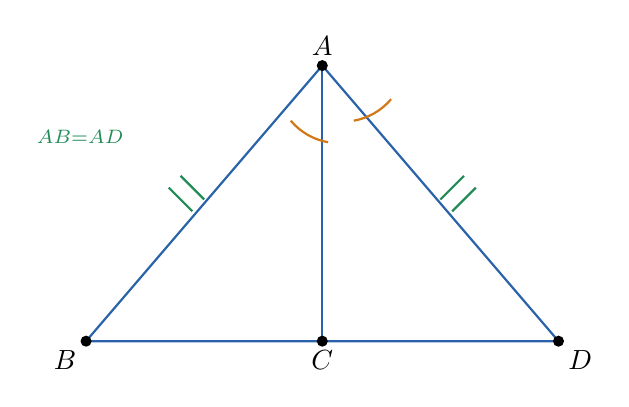
\begin{tikzpicture}[scale=1.0]
  \coordinate (A) at (3,3.5);
  \coordinate (B) at (0,0);
  \coordinate (D) at (6,0);
  \coordinate (C) at (3,0);
  \draw[thick, mainblue] (A)--(B)--(D)--cycle;
  \draw[thick, mainblue] (A)--(C);
  % 相等标记
  \draw[thick, tipgreen] (1.2,2.1)--(1.5,1.8);
  \draw[thick, tipgreen] (1.05,1.95)--(1.35,1.65);
  \draw[thick, tipgreen] (4.8,2.1)--(4.5,1.8);
  \draw[thick, tipgreen] (4.95,1.95)--(4.65,1.65);
  % 角平分线标记
  \draw[thick, examorange] (2.6,2.8) arc (220:260:0.8);
  \draw[thick, examorange] (3.4,2.8) arc (280:320:0.8);
  \fill (A) circle (2pt) node[above] {$A$};
  \fill (B) circle (2pt) node[below left] {$B$};
  \fill (C) circle (2pt) node[below] {$C$};
  \fill (D) circle (2pt) node[below right] {$D$};
  \node[tipgreen, left] at (0.6,2.6) {$\scriptstyle AB=AD$};
\end{tikzpicture}
\end{center}
\end{examplebox}

\noindent\textbf{证明：}

在 $\triangle ABC$ 和 $\triangle ADC$ 中：

$\because AB=AD$（已知），

$\angle BAC=\angle DAC$（$AC$ 平分 $\angle BAD$），

$AC=AC$（公共边），

$\therefore \triangle ABC \cong \triangle ADC$（SAS）。\hfill$\square$

\begin{tipbox}[方法总结]
本题考查\textbf{SAS 判定}。关键在于识别出"角平分线"提供了\textbf{夹角相等}的条件，加上公共边 $AC$，三条件齐全。这是最基础也最重要的全等证明模式。
\end{tipbox}

\vspace{6pt}

% ========== 例题2：全等证明（AAS） ==========
\begin{examplebox}[【例题2】全等三角形证明（AAS）]
\textbf{已知：}如图，$AB \parallel CD$，$AB=CD$，$E$ 是 $BD$ 的中点。

\textbf{求证：}$\triangle ABE \cong \triangle CDE$。

\begin{center}
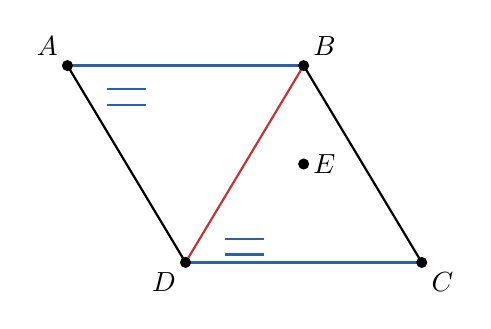
\begin{tikzpicture}[scale=1.0]
  \coordinate (A) at (0,2.5);
  \coordinate (B) at (3,2.5);
  \coordinate (C) at (4.5,0);
  \coordinate (D) at (1.5,0);
  \coordinate (E) at (3,1.25);
  \draw[thick, mainblue] (A)--(B);
  \draw[thick, mainblue] (C)--(D);
  \draw[thick] (A)--(D);
  \draw[thick] (B)--(C);
  \draw[thick, warnred] (B)--(D);
  \fill (A) circle (2pt) node[above left] {$A$};
  \fill (B) circle (2pt) node[above right] {$B$};
  \fill (C) circle (2pt) node[below right] {$C$};
  \fill (D) circle (2pt) node[below left] {$D$};
  \fill (E) circle (2pt) node[right] {$E$};
  % 平行标记
  \draw[thick, mainblue] (0.5,2.2)--(1.0,2.2);
  \draw[thick, mainblue] (0.5,2.0)--(1.0,2.0);
  \draw[thick, mainblue] (2.0,0.3)--(2.5,0.3);
  \draw[thick, mainblue] (2.0,0.1)--(2.5,0.1);
\end{tikzpicture}
\end{center}
\end{examplebox}

\noindent\textbf{证明：}

$\because AB \parallel CD$，

$\therefore \angle ABE=\angle CDE$，$\angle BAE=\angle DCE$（两直线平行，内错角相等）。

在 $\triangle ABE$ 和 $\triangle CDE$ 中：

$\because \angle ABE=\angle CDE$（已证），

$AB=CD$（已知），

$\angle BAE=\angle DCE$（已证），

$\therefore \triangle ABE \cong \triangle CDE$（AAS）。\hfill$\square$

\begin{tipbox}[方法总结]
本题的关键是利用\textbf{平行线}产生内错角，从而获得两对角相等。再结合已知的一对边相等，用 AAS 完成证明。注意：条件中"$E$ 是 $BD$ 的中点"实际上在 AAS 判定中没有用到，但它保证了 $\triangle ABE$ 和 $\triangle CDE$ 的位置关系。
\end{tipbox}

\vspace{6pt}

% ========== 例题3：相似证明（AA） ==========
\begin{examplebox}[【例题3】相似三角形证明（AA）]
\textbf{已知：}如图，在 $\triangle ABC$ 中，$\angle A=90°$，$AD \perp BC$ 于 $D$。

\textbf{求证：}$\triangle ABD \sim \triangle CBA \sim \triangle CAD$。

\begin{center}
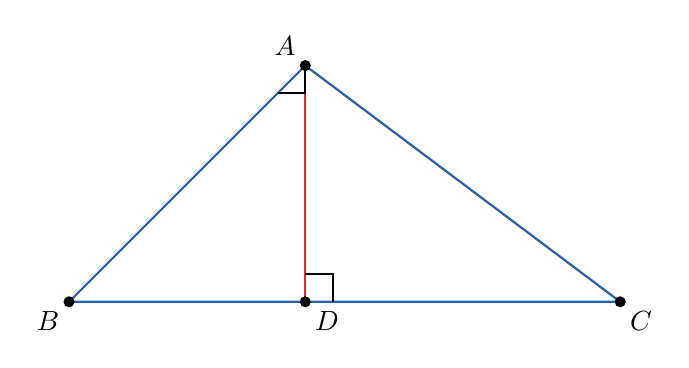
\begin{tikzpicture}[scale=1.0]
  \coordinate (A) at (0,3);
  \coordinate (B) at (-3,0);
  \coordinate (C) at (4,0);
  \coordinate (D) at (0,0);
  \draw[thick, mainblue] (A)--(B)--(C)--cycle;
  \draw[thick, warnred] (A)--(D);
  % 直角标记
  \draw[thick] (A)++(-0.35,-0.35)--++(0.35,0)--++(0,0.35);
  \draw[thick] (D)++(0,0.35)--++(0.35,0)--++(0,-0.35);
  \fill (A) circle (2pt) node[above left] {$A$};
  \fill (B) circle (2pt) node[below left] {$B$};
  \fill (C) circle (2pt) node[below right] {$C$};
  \fill (D) circle (2pt) node[below right] {$D$};
\end{tikzpicture}
\end{center}
\end{examplebox}

\noindent\textbf{证明：}

$\because \angle A=90°$，$AD \perp BC$，

$\therefore \angle ADB=\angle BAC=90°$。

在 $\triangle ABD$ 和 $\triangle CBA$ 中：

$\because \angle ADB=\angle CAB=90°$，

$\angle B=\angle B$（公共角），

$\therefore \triangle ABD \sim \triangle CBA$（AA）。

\medskip
同理，在 $\triangle CAD$ 和 $\triangle CBA$ 中：

$\because \angle ADC=\angle CAB=90°$，

$\angle C=\angle C$（公共角），

$\therefore \triangle CAD \sim \triangle CBA$（AA）。

$\therefore \triangle ABD \sim \triangle CBA \sim \triangle CAD$。\hfill$\square$

\begin{tipbox}[方法总结]
直角三角形斜边上的高将原三角形分成两个小三角形，这三个三角形\textbf{两两相似}。这是一个非常重要的基本图形，被称为"\textbf{射影定理的基本图}"。由此可得：
\[
AD^2 = BD \cdot DC, \quad AB^2 = BD \cdot BC, \quad AC^2 = CD \cdot BC
\]
\end{tipbox}

\vspace{6pt}

% ========== 例题4：利用相似求长度 ==========
\begin{examplebox}[【例题4】利用相似求线段长度]
\textbf{已知：}如图，$DE \parallel BC$，$AD=3$，$DB=2$，$BC=8$。

\textbf{求：}$DE$ 的长。

\begin{center}
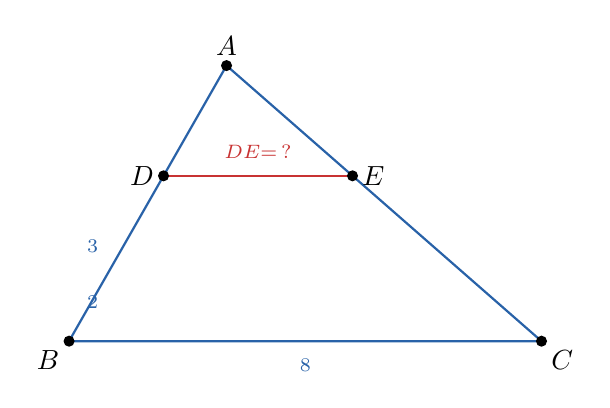
\begin{tikzpicture}[scale=1.0]
  \coordinate (A) at (2,3.5);
  \coordinate (B) at (0,0);
  \coordinate (C) at (6,0);
  \coordinate (D) at (1.2,2.1);
  \coordinate (E) at (3.6,2.1);
  \draw[thick, mainblue] (A)--(B)--(C)--cycle;
  \draw[thick, warnred] (D)--(E);
  % 标注
  \fill (A) circle (2pt) node[above] {$A$};
  \fill (B) circle (2pt) node[below left] {$B$};
  \fill (C) circle (2pt) node[below right] {$C$};
  \fill (D) circle (2pt) node[left] {$D$};
  \fill (E) circle (2pt) node[right] {$E$};
  \node[mainblue] at (0.3,1.2) {$\scriptstyle 3$};
  \node[mainblue] at (0.3,0.5) {$\scriptstyle 2$};
  \node[mainblue] at (3,-0.3) {$\scriptstyle 8$};
  \node[warnred] at (2.4,2.4) {$\scriptstyle DE=\,?$};
\end{tikzpicture}
\end{center}
\end{examplebox}

\noindent\textbf{解：}

$\because DE \parallel BC$，

$\therefore \triangle ADE \sim \triangle ABC$（AA：$\angle A$ 公共，$\angle ADE=\angle ABC$ 同位角相等），

$\therefore \dfrac{DE}{BC}=\dfrac{AD}{AB}$。

$\because AD=3$，$DB=2$，$\therefore AB=AD+DB=5$。

$\therefore \dfrac{DE}{8}=\dfrac{3}{5}$，

$\therefore DE=\dfrac{24}{5}=4.8$。\hfill$\square$

\begin{tipbox}[方法总结]
利用\textbf{平行线构造相似三角形}是求线段长度的基本方法。核心步骤：
\begin{enumerate}[nosep]
  \item 由平行线找到相似三角形（AA）；
  \item 写出对应边的比例关系；
  \item 代入已知数据，解方程。
\end{enumerate}
\end{tipbox}

\vspace{6pt}

% ========== 例题5：利用相似比求面积比 ==========
\begin{examplebox}[【例题5】利用相似求面积]
\textbf{已知：}如图，在 $\triangle ABC$ 中，$D$、$E$ 分别是 $AB$、$AC$ 的中点。

\textbf{求：}$S_{\triangle ADE} : S_{\triangle ABC}$。

\begin{center}
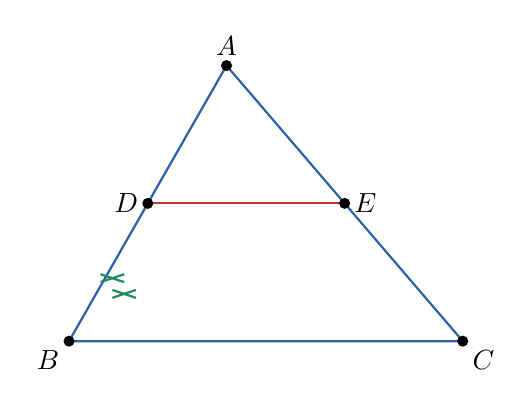
\begin{tikzpicture}[scale=1.0]
  \coordinate (A) at (2,3.5);
  \coordinate (B) at (0,0);
  \coordinate (C) at (5,0);
  \coordinate (D) at (1,1.75);
  \coordinate (E) at (3.5,1.75);
  \draw[thick, mainblue] (A)--(B)--(C)--cycle;
  \draw[thick, warnred] (D)--(E);
  \fill (A) circle (2pt) node[above] {$A$};
  \fill (B) circle (2pt) node[below left] {$B$};
  \fill (C) circle (2pt) node[below right] {$C$};
  \fill (D) circle (2pt) node[left] {$D$};
  \fill (E) circle (2pt) node[right] {$E$};
  % 中点标记
  \draw[thick, tipgreen] (0.4,0.85)--(0.7,0.75);
  \draw[thick, tipgreen] (0.55,0.65)--(0.85,0.55);
  \draw[thick, tipgreen] (0.7,0.85)--(0.4,0.75);
  \draw[thick, tipgreen] (0.85,0.65)--(0.55,0.55);
\end{tikzpicture}
\end{center}
\end{examplebox}

\noindent\textbf{解：}

$\because D$、$E$ 分别是 $AB$、$AC$ 的中点，

$\therefore DE$ 是 $\triangle ABC$ 的\textbf{中位线}，

$\therefore DE \parallel BC$，且 $DE=\dfrac{1}{2}BC$。

$\because DE \parallel BC$，

$\therefore \triangle ADE \sim \triangle ABC$（AA），

相似比 $k=\dfrac{DE}{BC}=\dfrac{1}{2}$。

$\therefore \dfrac{S_{\triangle ADE}}{S_{\triangle ABC}}=k^2=\left(\dfrac{1}{2}\right)^2=\dfrac{1}{4}$。

即 $S_{\triangle ADE}:S_{\triangle ABC}=1:4$。\hfill$\square$

\begin{tipbox}[方法总结]
三角形中位线定理（中位线平行于第三边且等于第三边的一半）是联系相似与面积的桥梁。记住：面积比 $=$ 相似比的\textbf{平方}。
\end{tipbox}

\vspace{6pt}

% ========== 例题6：四边形综合证明 ==========
\begin{examplebox}[【例题6】平行四边形综合证明]
\textbf{已知：}如图，在 $\square ABCD$ 中，$E$、$F$ 分别在 $AD$、$BC$ 上，且 $DE=BF$。

\textbf{求证：}$BE=DF$。

\begin{center}
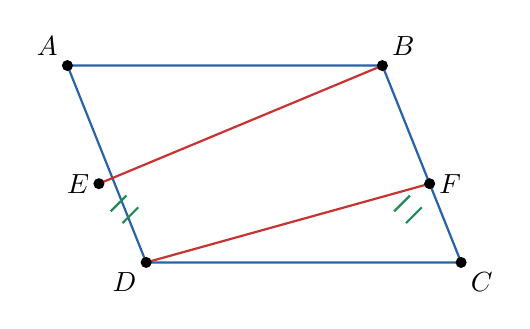
\begin{tikzpicture}[scale=1.0]
  \coordinate (A) at (0,2.5);
  \coordinate (B) at (4,2.5);
  \coordinate (C) at (5,0);
  \coordinate (D) at (1,0);
  \coordinate (E) at (0.4,1.0);
  \coordinate (F) at (4.6,1.0);
  \draw[thick, mainblue] (A)--(B)--(C)--(D)--cycle;
  \draw[thick, warnred] (B)--(E);
  \draw[thick, warnred] (D)--(F);
  \fill (A) circle (2pt) node[above left] {$A$};
  \fill (B) circle (2pt) node[above right] {$B$};
  \fill (C) circle (2pt) node[below right] {$C$};
  \fill (D) circle (2pt) node[below left] {$D$};
  \fill (E) circle (2pt) node[left] {$E$};
  \fill (F) circle (2pt) node[right] {$F$};
  % 等长标记
  \draw[thick, tipgreen] (0.7,0.5)--(0.9,0.7);
  \draw[thick, tipgreen] (0.55,0.65)--(0.75,0.85);
  \draw[thick, tipgreen] (4.3,0.5)--(4.5,0.7);
  \draw[thick, tipgreen] (4.15,0.65)--(4.35,0.85);
\end{tikzpicture}
\end{center}
\end{examplebox}

\noindent\textbf{证明：}

$\because ABCD$ 是平行四边形，

$\therefore AD \parallel BC$，$AD=BC$（平行四边形对边平行且相等）。

$\because DE=BF$，

$\therefore AE=AD-DE=BC-BF=CF$。

又 $\because AD \parallel BC$，

$\therefore AE \parallel CF$。

$\therefore$ 四边形 $AECF$ 是平行四边形（一组对边平行且相等）。

\medskip
同理，$\because DE=BF$，$DE \parallel BF$，

$\therefore$ 四边形 $BEDF$ 是平行四边形。

$\therefore BE=DF$（平行四边形对边相等）。\hfill$\square$

\begin{tipbox}[方法总结]
本题的关键思路是\textbf{证明四边形是平行四边形}，再利用对边相等得到结论。证明平行四边形时，"一组对边平行且相等"是最常用的判定方法。
\end{tipbox}

\vspace{6pt}

% ========== 例题7：辅助线应用（倍长中线） ==========
\begin{examplebox}[【例题7】辅助线应用——倍长中线]
\textbf{已知：}如图，在 $\triangle ABC$ 中，$AD$ 是 $BC$ 边上的中线，$AB=5$，$AC=3$。

\textbf{求：}$AD$ 的取值范围。

\begin{center}
\begin{tikzpicture}[scale=1.0]
  \coordinate (A) at (2,3.5);
  \coordinate (B) at (0,0);
  \coordinate (C) at (5,0);
  \coordinate (D) at (2.5,0);
  \coordinate (E) at (3,-3.5);
  \draw[thick, mainblue] (A)--(B)--(C)--cycle;
  \draw[thick, mainblue] (A)--(D);
  \draw[thick, dashed, dashgray] (D)--(E);
  \draw[thick, dashed, dashgray] (B)--(E);
  \draw[thick, dashed, warnred] (A)--(E);
  \fill (A) circle (2pt) node[above] {$A$};
  \fill (B) circle (2pt) node[below left] {$B$};
  \fill (C) circle (2pt) node[below right] {$C$};
  \fill (D) circle (2pt) node[below left] {$D$};
  \fill (E) circle (2pt) node[below right] {$E$};
\end{tikzpicture}
\end{center}
\end{examplebox}

\noindent\textbf{解：}

延长 $AD$ 至 $E$，使 $DE=AD$，连接 $BE$。

在 $\triangle ADB$ 和 $\triangle EDC$ 中：

$\because BD=DC$（$D$ 为中点），$AD=DE$（作图），$\angle ADB=\angle EDC$（对顶角），

$\therefore \triangle ADB \cong \triangle EDC$（SAS），

$\therefore AB=EC=5$，$AE=2AD$。

在 $\triangle ACE$ 中，由三角不等式：

$EC-AC < AE < EC+AC$，

即 $5-3 < 2AD < 5+3$，

$\therefore 1 < AD < 4$。\hfill$\square$

\begin{tipbox}[方法总结]
\textbf{倍长中线法}将 $AB$ 转移到 $CE$ 位置，使 $AB$、$AC$、$2AD$ 集中在同一三角形中。核心步骤：\textbf{一倍长、二连端、三全等、四转移}。遇到中线问题，优先考虑此法。
\end{tipbox}

\vspace{6pt}

% ========== 例题8：全等+相似综合 ==========
\begin{examplebox}[【例题8】全等与相似综合]
\textbf{已知：}如图，在 $\triangle ABC$ 中，$\angle BAC=90°$，$AB=AC$，$D$ 是 $BC$ 的中点，$E$ 是 $AC$ 上一点，$BE$ 交 $AD$ 于 $F$。

\textbf{求证：}$\triangle BDF \sim \triangle ADC$。

\begin{center}
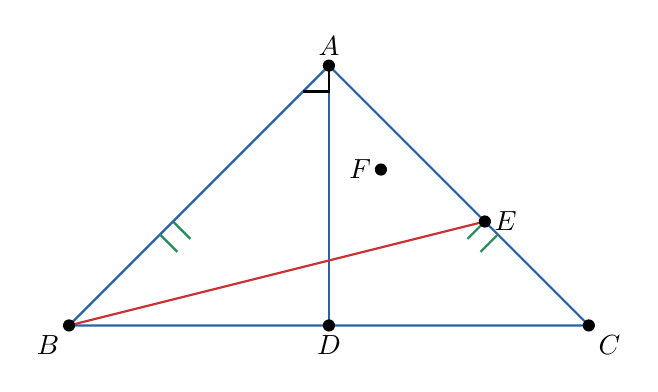
\begin{tikzpicture}[scale=1.1]
  \coordinate (A) at (3,3);
  \coordinate (B) at (0,0);
  \coordinate (C) at (6,0);
  \coordinate (D) at (3,0);
  \coordinate (E) at (4.8,1.2);
  \coordinate (F) at (3.6,1.8);
  \draw[thick, mainblue] (A)--(B)--(C)--cycle;
  \draw[thick, mainblue] (A)--(D);
  \draw[thick, warnred] (B)--(E);
  % 直角标记
  \draw[thick] (A)++(-0.3,-0.3)--++(0.3,0)--++(0,0.3);
  % 等长标记
  \draw[thick, tipgreen] (1.2,1.2)--(1.4,1.0);
  \draw[thick, tipgreen] (1.05,1.05)--(1.25,0.85);
  \draw[thick, tipgreen] (4.8,1.2)--(4.6,1.0);
  \draw[thick, tipgreen] (4.95,1.05)--(4.75,0.85);
  \fill (A) circle (2pt) node[above] {$A$};
  \fill (B) circle (2pt) node[below left] {$B$};
  \fill (C) circle (2pt) node[below right] {$C$};
  \fill (D) circle (2pt) node[below] {$D$};
  \fill (E) circle (2pt) node[right] {$E$};
  \fill (F) circle (2pt) node[left] {$F$};
\end{tikzpicture}
\end{center}
\end{examplebox}

\noindent\textbf{证明：}

$\because \angle BAC=90°$，$AB=AC$，

$\therefore \triangle ABC$ 是等腰直角三角形，

$\therefore \angle ABC=\angle ACB=45°$。

$\because D$ 是 $BC$ 的中点，$AB=AC$，

$\therefore AD \perp BC$（等腰三角形底边中点与顶点连线垂直于底边），

$\therefore \angle ADB=\angle ADC=90°$。

\medskip
在 $\triangle BDF$ 和 $\triangle ADC$ 中：

$\because \angle BDF=\angle ADC=90°$，

$\angle DBF=\angle DAC$（都等于 $45°$ 减去公共角 $\angle ADF$ 所对应的角，由 $\angle FBD=\angle FBA$，且 $\angle DBA=45°=\angle DCA$），

$\therefore \triangle BDF \sim \triangle ADC$（AA）。\hfill$\square$

\begin{tipbox}[方法总结]
本题综合运用了\textbf{等腰三角形性质}、\textbf{直角三角形性质}和\textbf{AA 相似判定}。关键是利用等腰直角三角形的特殊角（$45°$）来找到两对角相等。这类"全等 + 相似"的综合题在高中立体几何中经常出现。
\end{tipbox}

\vspace{6pt}

% ========== 例题9：几何与坐标系综合 ==========
\begin{examplebox}[【例题9】几何与坐标系综合]
\textbf{已知：}如图，在平面直角坐标系中，$A(0,4)$，$B(3,0)$，$C(6,0)$。

\textbf{求：}$\triangle ABC$ 的面积，以及 $AB$ 边上的高 $CH$ 的长。

\begin{center}
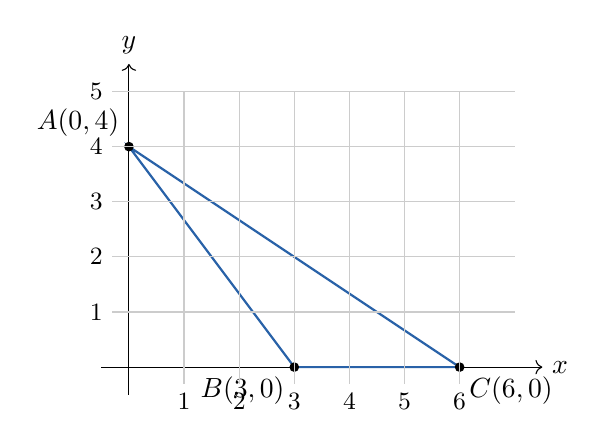
\begin{tikzpicture}[scale=0.7]
  \draw[->] (-0.5,0)--(7.5,0) node[right]{$x$};
  \draw[->] (0,-0.5)--(0,5.5) node[above]{$y$};
  \coordinate (A) at (0,4);
  \coordinate (B) at (3,0);
  \coordinate (C) at (6,0);
  \draw[thick, mainblue] (A)--(B)--(C)--cycle;
  \fill (A) circle (2.5pt) node[above left] {$A(0,4)$};
  \fill (B) circle (2.5pt) node[below left] {$B(3,0)$};
  \fill (C) circle (2.5pt) node[below right] {$C(6,0)$};
  % 坐标网格
  \foreach \x in {1,2,...,6} \draw[thin, gray!40] (\x,-0.3)--(\x,5);
  \foreach \y in {1,2,...,5} \draw[thin, gray!40] (-0.3,\y)--(7,\y);
  % 刻度
  \foreach \x in {1,2,...,6} \node[below] at (\x,-0.3) {\small\x};
  \foreach \y in {1,2,...,5} \node[left] at (-0.3,\y) {\small\y};
\end{tikzpicture}
\end{center}
\end{examplebox}

\noindent\textbf{解：}

$BC=6-3=3$，$BC$ 边上的高为 $A$ 到 $x$ 轴的距离，即 $4$。

$S_{\triangle ABC}=\dfrac{1}{2}\times 3\times 4=6$。

\medskip
求 $AB$ 边上的高 $CH$：

$AB=\sqrt{3^2+4^2}=5$（勾股定理），

$S_{\triangle ABC}=\dfrac{1}{2}\times AB\times CH$，

$\therefore 6=\dfrac{1}{2}\times 5\times CH$，

$\therefore CH=\dfrac{12}{5}=2.4$。\hfill$\square$

\begin{tipbox}[方法总结]
坐标系中的几何题，核心方法是：
\begin{enumerate}[nosep]
  \item 利用\textbf{坐标差}求线段长（勾股定理或水平/竖直距离）；
  \item 利用\textbf{面积法}求高——同一个三角形面积用两种底×高来表示，联立求解。
\end{enumerate}
"面积法"在高中数学中非常实用，务必掌握。
\end{tipbox}

\vspace{6pt}

% ========== 例题10：证明书写规范 ==========
\begin{examplebox}[【例题10】证明书写规范——完整示范]
\textbf{已知：}如图，$AB=CD$，$\angle ABC=\angle DCB$。

\textbf{求证：}$AC=BD$。

\begin{center}
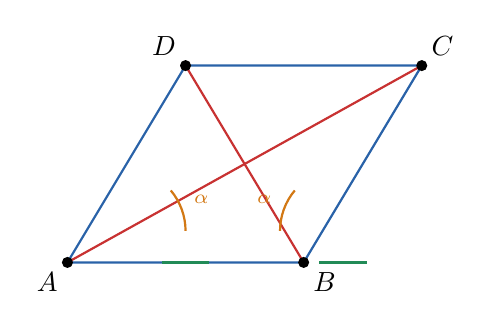
\begin{tikzpicture}[scale=1.0]
  \coordinate (A) at (0,0);
  \coordinate (B) at (3,0);
  \coordinate (C) at (4.5,2.5);
  \coordinate (D) at (1.5,2.5);
  \draw[thick, mainblue] (A)--(B)--(C)--(D)--cycle;
  \draw[thick, warnred] (A)--(C);
  \draw[thick, warnred] (B)--(D);
  \fill (A) circle (2pt) node[below left] {$A$};
  \fill (B) circle (2pt) node[below right] {$B$};
  \fill (C) circle (2pt) node[above right] {$C$};
  \fill (D) circle (2pt) node[above left] {$D$};
  % 角标记
  \draw[thick, examorange] (1.5,0.4) arc (0:40:0.8);
  \draw[thick, examorange] (2.7,0.4) arc (180:140:0.8);
  \node[examorange] at (1.7,0.8) {$\scriptstyle\alpha$};
  \node[examorange] at (2.5,0.8) {$\scriptstyle\alpha$};
  % 边标记
  \draw[thick, tipgreen] (1.2,0)--(1.5,0);
  \draw[thick, tipgreen] (1.5,0)--(1.8,0);
  \draw[thick, tipgreen] (3.2,0)--(3.5,0);
  \draw[thick, tipgreen] (3.5,0)--(3.8,0);
\end{tikzpicture}
\end{center}
\end{examplebox}

\noindent\textbf{证明：}

\textbf{【已知】}$AB=CD$，$\angle ABC=\angle DCB$。

\textbf{【求证】}$AC=BD$。

\medskip
在 $\triangle ABC$ 和 $\triangle DCB$ 中，

$\left\{\begin{array}{l}
AB=DC \quad \text{（已知）} \\[4pt]
\angle ABC=\angle DCB \quad \text{（已知）} \\[4pt]
BC=CB \quad \text{（公共边）}
\end{array}\right.$

$\therefore \triangle ABC \cong \triangle DCB$（SAS），

$\therefore AC=BD$（全等三角形对应边相等）。

$\square$

\begin{warnbox}[书写规范要点]
\begin{enumerate}[nosep]
  \item 证明开头明确写出"已知"和"求证"；
  \item 列条件时用\textbf{大括号}整齐排列，每条后面注明理由；
  \item 全等判定写在括号里（如 SAS、SSS、ASA、AAS、HL）；
  \item 最终结论前用 $\therefore$，以 $\square$ 结尾；
  \item 整体排版清晰，层次分明。
\end{enumerate}
\end{warnbox}

\newpage

% ============================================================
%  第三部分：应用题
% ============================================================
\section*{\textcolor{apppurple}{三、应用题}}

\begin{appbox}[【应用1】利用相似测量高度]
小明想测量学校旗杆的高度。他在地面上竖直立了一根 $1.5$ 米长的标杆，测得标杆的影长为 $1$ 米，同时测得旗杆的影长为 $8$ 米。已知测量时标杆和旗杆的影子在同一时刻产生。

\begin{center}
\begin{tikzpicture}[scale=0.8]
  % 旗杆
  \coordinate (A) at (0,0);
  \coordinate (B) at (0,5);
  \draw[thick, mainblue] (A)--(B);
  % 旗杆影子
  \draw[thick, dashgray] (A)--(5.5,0);
  \node[below] at (2.75,-0.2) {$\scriptstyle 8$ 米};
  % 标杆
  \coordinate (C) at (7,0);
  \coordinate (D) at (7,1.5);
  \draw[thick, examorange] (C)--(D);
  % 标杆影子
  \draw[thick, dashgray] (C)--(8,0);
  \node[below] at (7.5,-0.2) {$\scriptstyle 1$ 米};
  % 标注
  \node[mainblue, left] at (0,2.5) {$\scriptstyle h$};
  \node[examorange, right] at (7,0.75) {$\scriptstyle 1.5$};
  \fill (A) circle (2pt);
  \fill (B) circle (2pt) node[above] {旗杆顶};
  \fill (C) circle (2pt);
  \fill (D) circle (2pt) node[above] {杆顶};
  % 阳光线
  \draw[thin, gray, ->] (5.5,0.1)--(5.8,0.8);
  \draw[thin, gray, ->] (8,0.1)--(8.3,0.4);
\end{tikzpicture}
\end{center}

\textbf{（1）}旗杆有多高？

\textbf{（2）}如果某天旗杆的影长为 $10$ 米，标杆影长应该是多少？
\end{appbox}

\noindent\textbf{解：}

\textbf{（1）}同一时刻，阳光的入射角相同，旗杆和标杆与其影子构成的直角三角形相似。

$\therefore \dfrac{\text{旗杆高度}}{\text{旗杆影长}}=\dfrac{\text{标杆高度}}{\text{标杆影长}}$，

$\therefore \dfrac{h}{8}=\dfrac{1.5}{1}$，

$\therefore h=12$（米）。

答：旗杆高 $12$ 米。

\medskip
\textbf{（2）}$\dfrac{12}{10}=\dfrac{1.5}{\text{标杆影长}}$，

$\therefore$ 标杆影长 $=\dfrac{1.5\times 10}{12}=1.25$（米）。

答：标杆影长应为 $1.25$ 米。\hfill$\square$

\vspace{8pt}

\begin{appbox}[【应用2】利用相似计算不可达距离]
如图，为了测量河宽 $AB$，在河对岸选取一点 $C$，在河这岸选取 $A$、$D$ 两点，使得 $A$、$D$、$C$ 在同一直线上。再在 $AD$ 上选取点 $B$，测得 $AB=20$ 米，$BD=30$ 米。过 $B$ 作 $BE \parallel AC$，在 $BE$ 上取点 $E$，使得 $D$、$C$、$E$ 三点共线，测得 $BE=15$ 米。

\begin{center}
\begin{tikzpicture}[scale=0.7]
  \coordinate (A) at (0,0);
  \coordinate (B) at (3,0);
  \coordinate (D) at (7.5,0);
  \coordinate (C) at (5,3);
  \coordinate (E) at (7,2.25);
  \draw[thick, mainblue] (A)--(C);
  \draw[thick, mainblue] (A)--(D);
  \draw[thick, warnred] (B)--(E);
  \draw[thick] (D)--(C)--(E);
  % 标注
  \fill (A) circle (2pt) node[below left] {$A$};
  \fill (B) circle (2pt) node[below] {$B$};
  \fill (C) circle (2pt) node[above] {$C$};
  \fill (D) circle (2pt) node[below right] {$D$};
  \fill (E) circle (2pt) node[right] {$E$};
  \node at (1.5,-0.4) {$\scriptstyle 20$};
  \node at (5.25,-0.4) {$\scriptstyle 30$};
  \node[warnred, above] at (5,1.1) {$\scriptstyle 15$};
  % 河
  \draw[thick, blue!40] (-0.5,1.5)--(6.5,1.5);
  \node[blue!60] at (-0.5,1.8) {河};
\end{tikzpicture}
\end{center}

求河宽 $AC$ 的长。
\end{appbox}

\noindent\textbf{解：}

$\because BE \parallel AC$，

$\therefore \angle EBD=\angle CAD$，$\angle BED=\angle DCA$（两直线平行，内错角/同位角相等），

$\therefore \triangle BDE \sim \triangle ADC$（AA），

$\therefore \dfrac{BE}{AC}=\dfrac{BD}{AD}$。

$\because AD=AB+BD=20+30=50$，

$\therefore \dfrac{15}{AC}=\dfrac{30}{50}$，

$\therefore AC=\dfrac{15\times 50}{30}=25$（米）。

答：河宽 $AC$ 为 $25$ 米。\hfill$\square$

\vspace{8pt}

\begin{appbox}[【应用3】利用全等测量池塘宽度]
如图，要测量池塘两端 $A$、$B$ 的距离，先在平地上取一点 $C$，连接 $AC$ 并延长到 $D$，使 $CD=AC$；连接 $BC$ 并延长到 $E$，使 $CE=BC$。测得 $DE=18$ 米。

\begin{center}
\begin{tikzpicture}[scale=0.8]
  \coordinate (A) at (0,2.5);
  \coordinate (B) at (4,2.5);
  \coordinate (C) at (2,1);
  \coordinate (D) at (4,-0.5);
  \coordinate (E) at (0,-0.5);
  \draw[thick, blue!50] (A)--(B);
  \draw[thick, mainblue] (A)--(D);
  \draw[thick, mainblue] (B)--(E);
  \draw[thick, examorange] (D)--(E);
  % 标注
  \fill (A) circle (2pt) node[above left] {$A$};
  \fill (B) circle (2pt) node[above right] {$B$};
  \fill (C) circle (2pt) node[left] {$C$};
  \fill (D) circle (2pt) node[below right] {$D$};
  \fill (E) circle (2pt) node[below left] {$E$};
  \node at (3.25,-0.9) {$\scriptstyle DE=18$};
  % 池塘
  \draw[thick, blue!40, decorate, decoration={snake, amplitude=1.5pt, segment length=8pt}] (-0.5,2.8)--(4.5,2.8);
  \node[blue!60] at (2,3.1) {池塘};
  % 等长标记
  \draw[thick, tipgreen] (0.8,1.9)--(1.0,1.7);
  \draw[thick, tipgreen] (1.4,1.4)--(1.6,1.2);
  \draw[thick, tipgreen] (1.2,1.8)--(1.4,1.6);
  \draw[thick, tipgreen] (1.8,1.3)--(2.0,1.1);
  \draw[thick, tipgreen] (3.2,1.9)--(3.0,1.7);
  \draw[thick, tipgreen] (2.6,1.4)--(2.4,1.2);
  \draw[thick, tipgreen] (2.8,1.8)--(2.6,1.6);
  \draw[thick, tipgreen] (2.2,1.3)--(2.0,1.1);
\end{tikzpicture}
\end{center}

求 $AB$ 的长。
\end{appbox}

\noindent\textbf{解：}

在 $\triangle ABC$ 和 $\triangle DEC$ 中：

$\because AC=DC$（已知），$BC=EC$（已知），$\angle ACB=\angle DCE$（对顶角），

$\therefore \triangle ABC \cong \triangle DEC$（SAS），

$\therefore AB=DE=18$（米）。

答：$AB$ 的长为 $18$ 米。\hfill$\square$

\begin{tipbox}[方法总结]
利用\textbf{全等三角形}测量不可达距离，是全等知识最经典的实际应用。关键是通过"延长中点"构造全等，将不可测量的 $AB$ 转化为可测量的 $DE$。
\end{tipbox}

\newpage

% ============================================================
%  第四部分：课堂练习
% ============================================================
\section*{\textcolor{tipgreen}{四、课堂练习}}

\begin{enumerate}[leftmargin=2em, itemsep=10pt]

\item 如图，在 $\triangle ABC$ 和 $\triangle DEF$ 中，$AB=DE$，$\angle B=\angle E$，$BC=EF$。求证：$\triangle ABC \cong \triangle DEF$。

\begin{center}
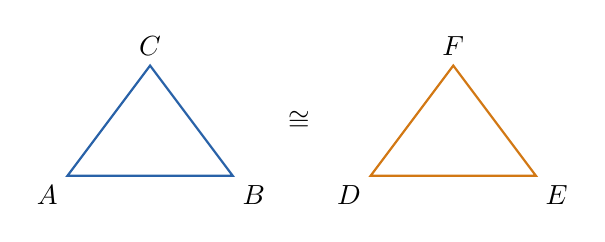
\begin{tikzpicture}[scale=0.7]
  \coordinate (A) at (0,0);
  \coordinate (B) at (3,0);
  \coordinate (C) at (1.5,2);
  \draw[thick, mainblue] (A)--(B)--(C)--cycle;
  \node[below left] at (A) {$A$};
  \node[below right] at (B) {$B$};
  \node[above] at (C) {$C$};
  \node at (4.2,1) {$\cong$};
  \coordinate (D) at (5.5,0);
  \coordinate (E) at (8.5,0);
  \coordinate (F) at (7,2);
  \draw[thick, examorange] (D)--(E)--(F)--cycle;
  \node[below left] at (D) {$D$};
  \node[below right] at (E) {$E$};
  \node[above] at (F) {$F$};
\end{tikzpicture}
\end{center}

\item 如图，在 $\triangle ABC$ 中，$D$ 是 $AB$ 上一点，$\angle ACD=\angle B$。求证：$\triangle ACD \sim \triangle ABC$，并求 $\dfrac{AD}{AC}$（已知 $AD=4$，$AC=6$）。

\begin{center}
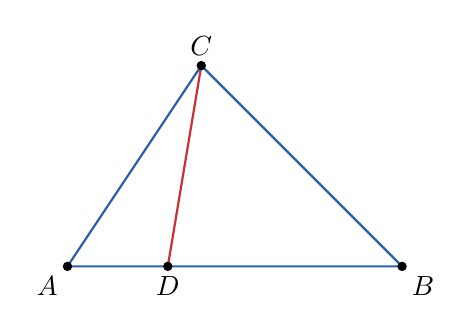
\begin{tikzpicture}[scale=0.85]
  \coordinate (A) at (0,0);
  \coordinate (B) at (5,0);
  \coordinate (C) at (2,3);
  \coordinate (D) at (1.5,0);
  \draw[thick, mainblue] (A)--(B)--(C)--cycle;
  \draw[thick, warnred] (C)--(D);
  \fill (A) circle (2pt) node[below left] {$A$};
  \fill (B) circle (2pt) node[below right] {$B$};
  \fill (C) circle (2pt) node[above] {$C$};
  \fill (D) circle (2pt) node[below] {$D$};
\end{tikzpicture}
\end{center}

\item 如图，$AB \parallel CD$，$AC$ 与 $BD$ 交于点 $O$，$AO=3$，$CO=5$，$BO=4$。求 $DO$ 的长。

\begin{center}
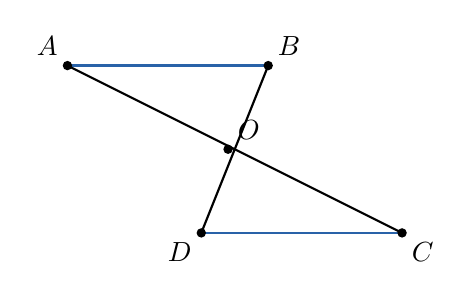
\begin{tikzpicture}[scale=0.85]
  \coordinate (A) at (0,2.5);
  \coordinate (B) at (3,2.5);
  \coordinate (C) at (5,0);
  \coordinate (D) at (2,0);
  \coordinate (O) at (2.4,1.25);
  \draw[thick, mainblue] (A)--(B);
  \draw[thick, mainblue] (C)--(D);
  \draw[thick] (A)--(C);
  \draw[thick] (B)--(D);
  \fill (A) circle (2pt) node[above left] {$A$};
  \fill (B) circle (2pt) node[above right] {$B$};
  \fill (C) circle (2pt) node[below right] {$C$};
  \fill (D) circle (2pt) node[below left] {$D$};
  \fill (O) circle (2pt) node[above right] {$O$};
\end{tikzpicture}
\end{center}

\item 如图，在 $\square ABCD$ 中，对角线 $AC$ 和 $BD$ 交于点 $O$，$E$ 是 $OA$ 的中点，$F$ 是 $OC$ 的中点。求证：$BE=DF$。

\begin{center}
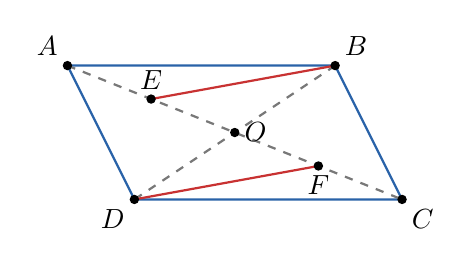
\begin{tikzpicture}[scale=0.85]
  \coordinate (A) at (0,2);
  \coordinate (B) at (4,2);
  \coordinate (C) at (5,0);
  \coordinate (D) at (1,0);
  \coordinate (O) at (2.5,1);
  \coordinate (E) at (1.25,1.5);
  \coordinate (F) at (3.75,0.5);
  \draw[thick, mainblue] (A)--(B)--(C)--(D)--cycle;
  \draw[thick, dashed, dashgray] (A)--(C);
  \draw[thick, dashed, dashgray] (B)--(D);
  \draw[thick, warnred] (B)--(E);
  \draw[thick, warnred] (D)--(F);
  \fill (A) circle (2pt) node[above left] {$A$};
  \fill (B) circle (2pt) node[above right] {$B$};
  \fill (C) circle (2pt) node[below right] {$C$};
  \fill (D) circle (2pt) node[below left] {$D$};
  \fill (O) circle (2pt) node[right] {$O$};
  \fill (E) circle (2pt) node[above] {$E$};
  \fill (F) circle (2pt) node[below] {$F$};
\end{tikzpicture}
\end{center}

\item 如图，$\triangle ABC$ 中，$\angle C=90°$，$CD \perp AB$ 于 $D$，$AC=6$，$BC=8$。求 $CD$ 的长。

\begin{center}
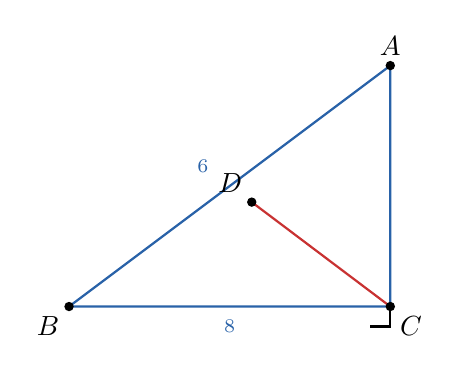
\begin{tikzpicture}[scale=0.85]
  \coordinate (A) at (0,3.6);
  \coordinate (B) at (-4.8,0);
  \coordinate (C) at (0,0);
  \coordinate (D) at (-2.07,1.56);
  \draw[thick, mainblue] (A)--(B)--(C)--cycle;
  \draw[thick, warnred] (C)--(D);
  \draw[thick] (C)++(-0.3,-0.3)--++(0.3,0)--++(0,0.3);
  \fill (A) circle (2pt) node[above] {$A$};
  \fill (B) circle (2pt) node[below left] {$B$};
  \fill (C) circle (2pt) node[below right] {$C$};
  \fill (D) circle (2pt) node[above left] {$D$};
  \node[mainblue] at (-2.8,2.1) {$\scriptstyle 6$};
  \node[mainblue] at (-2.4,-0.3) {$\scriptstyle 8$};
\end{tikzpicture}
\end{center}

\item 如图，在 $\triangle ABC$ 中，$D$、$E$ 分别是 $AB$、$AC$ 上的点，$DE \parallel BC$，$AD=2$，$DB=3$，$\triangle ABC$ 的面积为 $25$。求 $\triangle ADE$ 的面积。

\begin{center}
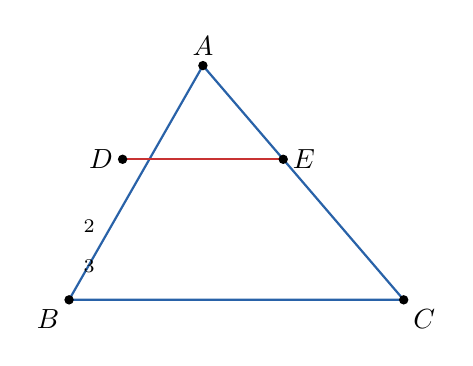
\begin{tikzpicture}[scale=0.85]
  \coordinate (A) at (2,3.5);
  \coordinate (B) at (0,0);
  \coordinate (C) at (5,0);
  \coordinate (D) at (0.8,2.1);
  \coordinate (E) at (3.2,2.1);
  \draw[thick, mainblue] (A)--(B)--(C)--cycle;
  \draw[thick, warnred] (D)--(E);
  \fill (A) circle (2pt) node[above] {$A$};
  \fill (B) circle (2pt) node[below left] {$B$};
  \fill (C) circle (2pt) node[below right] {$C$};
  \fill (D) circle (2pt) node[left] {$D$};
  \fill (E) circle (2pt) node[right] {$E$};
  \node at (0.3,1.1) {$\scriptstyle 2$};
  \node at (0.3,0.5) {$\scriptstyle 3$};
\end{tikzpicture}
\end{center}

\item 如图，在 $\triangle ABC$ 中，$AB=AC$，$\angle A=36°$，$BD$ 平分 $\angle ABC$。求证：$\triangle BCD \sim \triangle ABC$。

\begin{center}
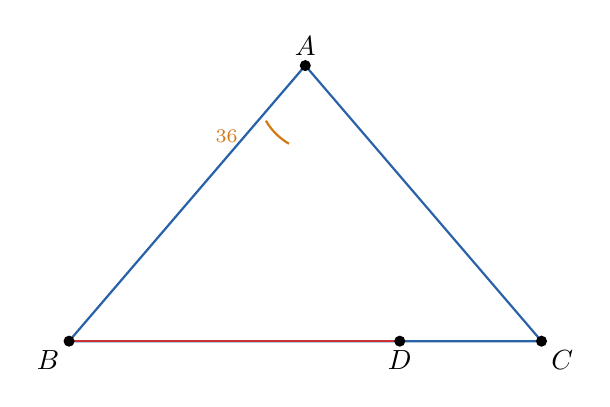
\begin{tikzpicture}[scale=1.0]
  \coordinate (A) at (3,3.5);
  \coordinate (B) at (0,0);
  \coordinate (C) at (6,0);
  \coordinate (D) at (4.2,0);
  \draw[thick, mainblue] (A)--(B)--(C)--cycle;
  \draw[thick, warnred] (B)--(D);
  \fill (A) circle (2pt) node[above] {$A$};
  \fill (B) circle (2pt) node[below left] {$B$};
  \fill (C) circle (2pt) node[below right] {$C$};
  \fill (D) circle (2pt) node[below] {$D$};
  % 角标记
  \draw[thick, examorange] (2.5,2.8) arc (210:240:0.8);
  \node[examorange] at (2.0,2.6) {$\scriptstyle 36°$};
\end{tikzpicture}
\end{center}

\item 如图，在平面直角坐标系中，$O(0,0)$，$A(4,0)$，$B(4,3)$。$P$ 是 $OB$ 的中点。求 $\triangle OAP$ 的面积和 $AP$ 的长。

\begin{center}
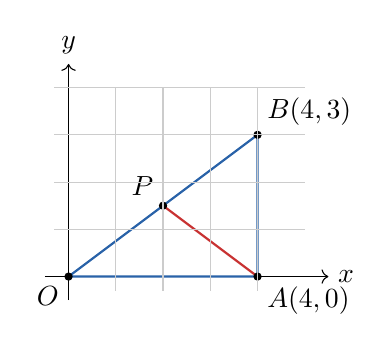
\begin{tikzpicture}[scale=0.6]
  \draw[->] (-0.5,0)--(5.5,0) node[right]{$x$};
  \draw[->] (0,-0.5)--(0,4.5) node[above]{$y$};
  \coordinate (O) at (0,0);
  \coordinate (A) at (4,0);
  \coordinate (B) at (4,3);
  \coordinate (P) at (2,1.5);
  \draw[thick, mainblue] (O)--(A)--(B)--cycle;
  \draw[thick, warnred] (A)--(P);
  \fill (O) circle (2.5pt) node[below left] {$O$};
  \fill (A) circle (2.5pt) node[below right] {$A(4,0)$};
  \fill (B) circle (2.5pt) node[above right] {$B(4,3)$};
  \fill (P) circle (2.5pt) node[above left] {$P$};
  \foreach \x in {1,...,4} \draw[thin, gray!40] (\x,-0.3)--(\x,4);
  \foreach \y in {1,...,4} \draw[thin, gray!40] (-0.3,\y)--(5,\y);
\end{tikzpicture}
\end{center}

\end{enumerate}

% ============================================================
%  参考答案
% ============================================================
\vspace{10pt}

\begin{knowledgebox}[参考答案]

\textbf{第1题：}

在 $\triangle ABC$ 和 $\triangle DEF$ 中，$AB=DE$，$\angle B=\angle E$，$BC=EF$，

$\therefore \triangle ABC \cong \triangle DEF$（SAS）。

\medskip
\textbf{第2题：}

在 $\triangle ACD$ 和 $\triangle ABC$ 中，$\angle A=\angle A$（公共角），$\angle ACD=\angle B$（已知），

$\therefore \triangle ACD \sim \triangle ABC$（AA），

$\therefore \dfrac{AD}{AC}=\dfrac{AC}{AB}$，即 $\dfrac{AD}{AC}=\dfrac{6}{AB}$。

由 $\dfrac{AD}{AC}=\dfrac{AC}{AB}$ 得 $AC^2=AD\cdot AB$，即 $36=4\cdot AB$，$AB=9$。

$\therefore \dfrac{AD}{AC}=\dfrac{4}{6}=\dfrac{2}{3}$。

\medskip
\textbf{第3题：}

$\because AB \parallel CD$，$\therefore \triangle AOB \sim \triangle COD$（AA），

$\therefore \dfrac{AO}{CO}=\dfrac{BO}{DO}$，即 $\dfrac{3}{5}=\dfrac{4}{DO}$，

$\therefore DO=\dfrac{20}{3}$。

\medskip
\textbf{第4题：}

$\because ABCD$ 是平行四边形，$O$ 是对角线交点，

$\therefore OA=OC$，$OB=OD$（平行四边形对角线互相平分）。

$\because E$ 是 $OA$ 中点，$F$ 是 $OC$ 中点，$\therefore OE=OF=\dfrac{1}{2}OA$。

在 $\triangle BOE$ 和 $\triangle DOF$ 中，$OB=OD$，$OE=OF$，$\angle BOE=\angle DOF$（对顶角），

$\therefore \triangle BOE \cong \triangle DOF$（SAS），$\therefore BE=DF$。

\medskip
\textbf{第5题：}

$AB=\sqrt{6^2+8^2}=10$。

$S_{\triangle ABC}=\dfrac{1}{2}\times 6\times 8=24$。

$S_{\triangle ABC}=\dfrac{1}{2}\times AB\times CD=\dfrac{1}{2}\times 10\times CD$，

$\therefore CD=\dfrac{48}{10}=4.8$。

\medskip
\textbf{第6题：}

$\because DE \parallel BC$，$\therefore \triangle ADE \sim \triangle ABC$（AA），

相似比 $k=\dfrac{AD}{AB}=\dfrac{2}{2+3}=\dfrac{2}{5}$，

$\therefore \dfrac{S_{\triangle ADE}}{S_{\triangle ABC}}=k^2=\dfrac{4}{25}$，

$\therefore S_{\triangle ADE}=\dfrac{4}{25}\times 25=4$。

\medskip
\textbf{第7题：}

$\because AB=AC$，$\angle A=36°$，$\therefore \angle ABC=\angle ACB=72°$。

$\because BD$ 平分 $\angle ABC$，$\therefore \angle ABD=\angle DBC=36°$。

在 $\triangle BCD$ 中，$\angle BDC=180°-72°-36°=72°$。

在 $\triangle BCD$ 和 $\triangle ACB$ 中，$\angle BCD=\angle ACB=72°$（公共角），$\angle DBC=\angle CAB=36°$，

$\therefore \triangle BCD \sim \triangle ACB$（AA）。

\medskip
\textbf{第8题：}

$\because P$ 是 $OB$ 的中点，$B(4,3)$，$\therefore P(2,1.5)$。

$OA=4$，$P$ 到 $x$ 轴距离 $=1.5$，

$S_{\triangle OAP}=\dfrac{1}{2}\times 4\times 1.5=3$。

$AP=\sqrt{(4-2)^2+(0-1.5)^2}=\sqrt{4+2.25}=\sqrt{6.25}=2.5$。

\end{knowledgebox}

\vfill
\begin{center}
\small\textcolor{gray}{本讲义仅供教学参考，例题可根据学生水平调整难度。}
\end{center}

\end{document}
